\documentclass[11pt]{article}
\usepackage[margin=1in]{geometry}
\usepackage{amsmath, amssymb}
\usepackage{graphicx}
\usepackage{booktabs}
\usepackage{parskip}
\usepackage{hyperref}

\title{Exp C: does the model's pre-decoding entropy track its own decoder $\beta$?}
\author{}
\date{\today}

\begin{document}
\maketitle

\section{Question}

The project proposal hypothesizes (\texttt{decoding-modeling.tex}):
\emph{language models form a belief about their own decoding parameters by
conditioning on the text they have generated}.  This experiment tests that
hypothesis directly: holding the prompt fixed, vary $\beta_{\mathrm{dec}}$
during self-generation and ask whether the model's pre-decoding entropy
$H(\mathrm{softmax}(\ell_t))$ at late steps reflects the decoder
$\beta_{\mathrm{dec}}$ in use.

\section{Setup}

Qwen-2.5-3B base, 32 prompts (\texttt{src/decoding\_decoding/prompts.py}),
each truncated to its first 10 tokens.  Generate 150 tokens per prompt at
three $\beta_{\mathrm{dec}}$ settings:
\[
\beta_{\mathrm{dec}} \in \{0.5\;(T=2.0),\ 1.0\;(T=1.0),\ 2.0\;(T=0.5)\}.
\]
At each step, record $H(\mathrm{softmax}(\ell_t))$ \emph{before} the decoder
applies $\beta_{\mathrm{dec}}$.  Late-window aggregation: per-prompt mean
$H$ over steps 80--149.

\section{First-look result}

\begin{figure}[h]
\centering
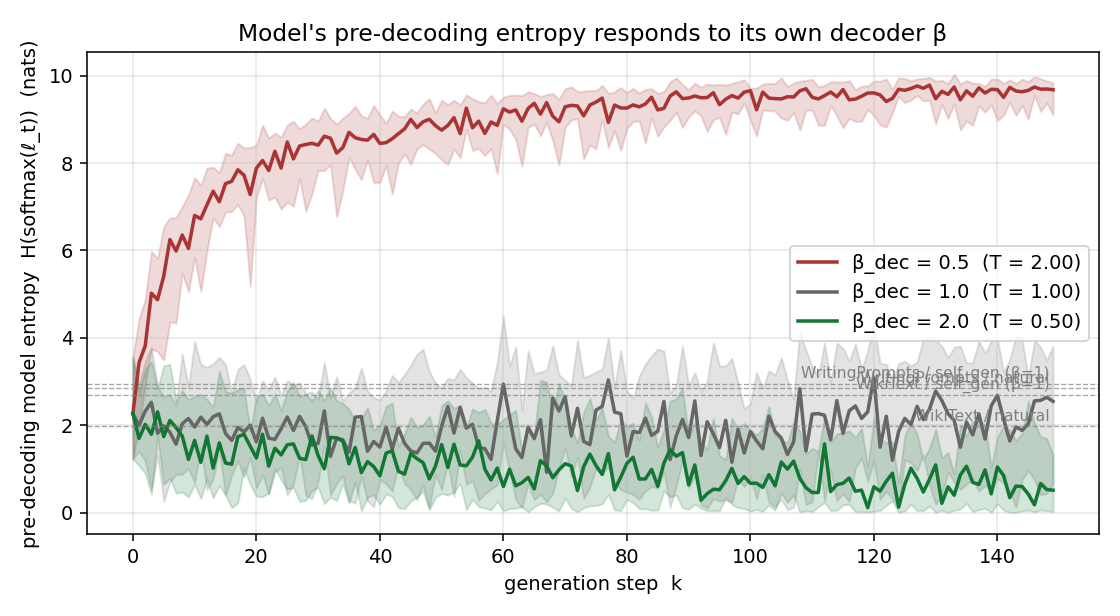
\includegraphics[width=0.92\linewidth]{F_ep_1_entropy_trajectory.png}
\caption{Median $H(t)$ per condition, IQR shaded.  Dashed grey lines mark
mean entropies of real natural text from the earlier natural\_text
experiment (Wikipedia $\approx 1.98$, WritingPrompts $\approx 2.85$ nats).}
\label{fig:exp-c-traj}
\end{figure}

\begin{table}[h]
\centering
\caption{Late-window (steps 80--149) pre-decoding entropy per
$\beta_{\mathrm{dec}}$, with per-prompt paired difference.}
\begin{tabular}{lcc}
\toprule
condition                       & late-window $H$ mean (nats) $\pm$ SE & paired diff vs $\beta=2.0$ \\
\midrule
$\beta_{\mathrm{dec}} = 0.5$    & $9.216 \pm 0.052$ & $+8.045 \pm 0.115$ ($t = +69.7$, $n_+ = 32/32$) \\
$\beta_{\mathrm{dec}} = 1.0$    & $2.168 \pm 0.186$ & $+1.00$                                       \\
$\beta_{\mathrm{dec}} = 2.0$    & $1.172 \pm 0.109$ & ---                                            \\
\bottomrule
\end{tabular}
\end{table}

The late-window entropy moves $\approx 8$ nats (factor $\approx 3000$ in
effective vocabulary) between $\beta_{\mathrm{dec}}=0.5$ and
$\beta_{\mathrm{dec}}=2.0$.  Every one of 32 prompts orders the same way.

\paragraph{Three observations before we believe the headline.}

\begin{enumerate}
\item Natural high-entropy human writing (WritingPrompts/natural) sits at
$H \approx 2.85$ nats --- nowhere near the 9.2 nats seen here.  So this is
not the model "reading off high-T-like content"; this is a regime that
only off-distribution self-sampling reaches.

\item Inspection of $\beta=0.5$ generations (Figure \ref{fig:exp-c-text})
shows pure token salad: code keywords, foreign-language fragments, URL
slugs, random named entities.  $\beta=1.0$ generations are coherent
English.  $\beta=2.0$ generations are also coherent English, more compressed
toward common factual phrasing.

\item The entropy trajectory at $\beta=0.5$ climbs monotonically from
$\approx 2$ at step~0 to $\approx 9$ at step~80: classic compounding
off-distribution drift, where each random token makes the next context less
parseable and the next sample yet more random.
\end{enumerate}

\begin{figure}[h]
\centering
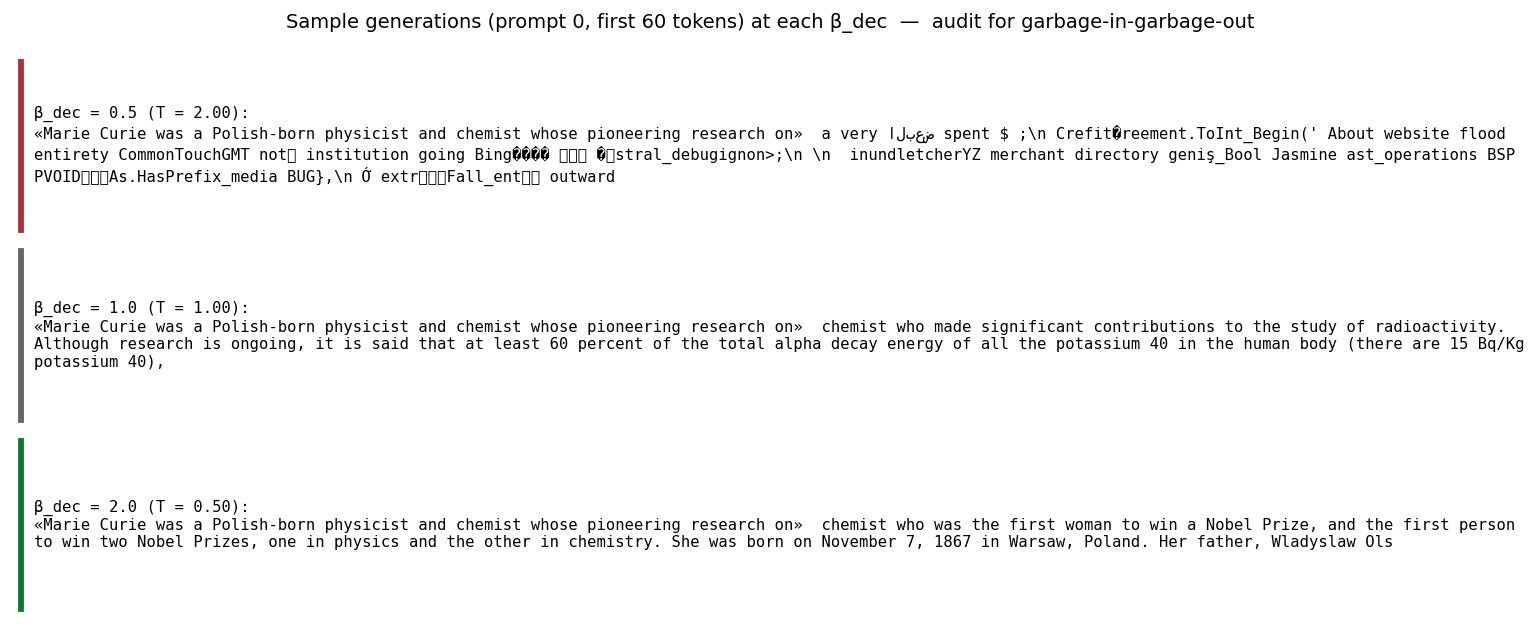
\includegraphics[width=0.92\linewidth]{F_ep_3_sample_generations.png}
\caption{First 60 sampled tokens for prompt 0 (Marie Curie) at each
$\beta_{\mathrm{dec}}$.  $\beta=0.5$ generation degrades to token salad
within $\approx 20$ steps.}
\label{fig:exp-c-text}
\end{figure}

These three points raise an obvious alternative: the 8-nat effect is
\emph{garbage-in, garbage-out} --- the model is uncertain because its
context is incoherent, not because it has formed a "belief" that the
decoder is set to high $T$.

\section{Swap-prefix control}

To disambiguate, we hold the early prefix's generation regime fixed and
\emph{switch} the sampler $\beta$ at step 80.  If the model truly has a
belief about $\beta_{\mathrm{dec}}$ that updates on recent tokens, then
switching to $\beta=1.0$ at step 80 should pull late-window $H$ down to the
$\beta_{\mathrm{dec}}=1.0$ baseline ($\approx 2$ nats) within $\sim 20$
tokens.  Five conditions, same 32 prompts:

\begin{itemize}
\item \texttt{pre05\_post05} --- $\beta = 0.5$ throughout (no switch, control).
\item \texttt{pre05\_post10} --- $\beta = 0.5 \to 1.0$ at step 80.
\textbf{This is the decisive comparison.}
\item \texttt{pre05\_post20} --- $\beta = 0.5 \to 2.0$ at step 80.
\item \texttt{pre20\_post05} --- $\beta = 2.0 \to 0.5$ at step 80 (mirror).
\item \texttt{pre20\_post20} --- $\beta = 2.0$ throughout (control).
\end{itemize}

\begin{figure}[h]
\centering
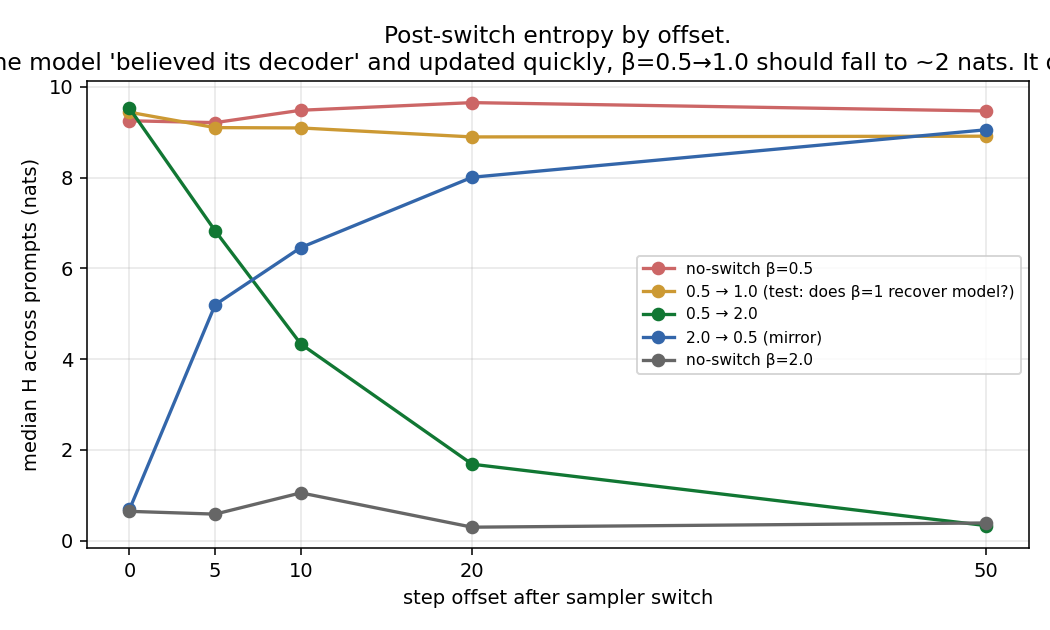
\includegraphics[width=0.92\linewidth]{F_ep_5_swap_recovery.png}
\caption{Median pre-decoding $H$ at offsets $+0, +5, +10, +20, +50$ after
the sampler switch.  Critical observation: \emph{the orange line
(\texttt{pre05\_post10}) does not fall} --- the model does not recover
coherence when the sampler switches to $\beta=1.0$.}
\label{fig:exp-c-swap}
\end{figure}

\begin{table}[h]
\centering
\caption{Pre-switch median $H$ and post-switch median $H$ at step offsets
from the switch.}
\begin{tabular}{lcrrrrrr}
\toprule
condition           & $\beta_{\mathrm{pre}}\!\to\!\beta_{\mathrm{post}}$ & pre-med & +0  & +5  & +10 & +20 & +50 \\
\midrule
\texttt{pre05\_post05} & $0.5 \to 0.5$ (no switch) & 8.42 & 9.26 & 9.21 & 9.49 & 9.66 & 9.47 \\
\texttt{pre05\_post10} & $0.5 \to 1.0$              & 8.56 & 9.44 & 9.10 & 9.10 & 8.90 & 8.92 \\
\texttt{pre05\_post20} & $0.5 \to 2.0$              & 8.57 & 9.53 & 6.83 & 4.33 & 1.68 & 0.33 \\
\texttt{pre20\_post05} & $2.0 \to 0.5$              & 1.21 & 0.69 & 5.20 & 6.46 & 8.01 & 9.06 \\
\texttt{pre20\_post20} & $2.0 \to 2.0$ (no switch) & 1.29 & 0.64 & 0.58 & 1.05 & 0.30 & 0.39 \\
\bottomrule
\end{tabular}
\end{table}

\paragraph{What this shows.}

\begin{itemize}
\item \texttt{pre05\_post10}: switching the sampler from $\beta=0.5$ to
$\beta=1.0$ leaves median $H$ essentially unchanged ($8.56 \to 8.92$ at
step $+50$).  The model does \emph{not} update its predictions to match
the new sampling regime over even 50 tokens of new evidence.

\item \texttt{pre05\_post20}: switching to $\beta=2.0$ \emph{does} recover
coherence over $\sim 20$ tokens.  But this recovery is explained by the
mechanism of $\beta=2$ sampling itself --- $\beta=2$ forces a top-1
selection from $\mathrm{softmax}(\beta \cdot \ell_t)$, which under a flat
$\ell_t$ still picks the highest-probability token (typically a common safe
continuation like punctuation, common articles, frequent function words);
those tokens then \emph{re-anchor} the context to in-distribution English.
This is not the model "updating its belief"; it is the sampler injecting
in-distribution tokens that gradually overwrite the bad prefix.
\end{itemize}

The decisive comparison \texttt{pre05\_post10} falsifies a strong form of
the "decoder-belief" framing.  If model-belief-about-$\beta$ were a fast
posterior update on recent sampled tokens, switching the sampler should be
visible within a handful of tokens.  It is not.

\section{What survives}

A weak form of the framing remains testable and may still be true, but is
not established by this experiment:

\begin{itemize}
\item At $\beta_{\mathrm{dec}}=2.0$ self-generation, late-window
$H \approx 1.17$ nats --- \emph{lower} than the model's entropy on real
WikiText ($1.98$ nats from \texttt{natural\_text/macros.tex}).  This
$\approx 0.8$-nat gap is consistent with the model sharpening below what
the natural content alone would justify, when its prefix matches the
$\beta=2$ regime.  But it is also consistent with $\beta=2$ generation
producing especially predictable content (top-1 sampling produces
high-frequency tokens), so this gap is suggestive, not decisive.
\item The earlier natural-text experiment found a small calibration offset
on real creative writing ($\Delta\log\hat\beta \approx -0.24$, $t = -3.8$).
That offset, on real human text, is a much weaker but cleaner signal than
the Exp C numbers and is the surviving load-bearing positive evidence for
the project's framing.
\end{itemize}

\section{Bottom line}

\begin{itemize}
\item The 8-nat entropy spread between $\beta_{\mathrm{dec}}=0.5$ and
$\beta_{\mathrm{dec}}=2.0$ self-generation is mostly the model
\emph{losing coherence} as its own off-distribution sampling decoheres the
context.  It is not a posterior on $\beta_{\mathrm{dec}}$.
\item The swap-prefix control confirms this: switching the sampler from
$\beta=0.5$ to $\beta=1.0$ does not pull $H$ back to the $\beta=1.0$
baseline over 50 tokens.  A model with a fast posterior on its decoder
would recover.
\item The project's framing must scope down: the model's distribution does
not aggressively update on the apparent decoder of its own generated
prefix at the timescales tested here.  Smaller signals --- e.g.\ the
WritingPrompts/natural offset from the natural\_text experiment, or the
$\sim 0.8$-nat sharpening below WikiText at $\beta=2.0$ --- are the
remaining candidates for clean "decoder-belief" evidence and need a
different experimental design to isolate.
\end{itemize}

\end{document}
